% References:
%   [1] https://tex.stackexchange.com/questions/118069/how-to-draw-an-euler-angle-rotation-sequence-with-tikz
%   [2] https://tex.stackexchange.com/questions/218354/i-want-to-draw-a-dot-small-sphere-in-a-tikz-3d-plot

% ---------
% Preamble.
% ---------

% Document type.
\documentclass{article}

% Import custom style.
\usepackage{../.preamble/tikz_diagrams_template}

% Color theme (black, red, blue, green, orange, purple, gold).
\colortheme{blue}

% ---------
% Document.
% ---------

\begin{document}

    % Sets viewing orientation (declination/rotation) of 3D coordinate system.
    \tdplotsetmaincoords{90}{0}

    % Change rotation matrix to use 3-2-1 sequence.
    \tdseteulerxyz

    % -----------------
    % TikZ environment.
    % -----------------

    \begin{tikzpicture}[tdplot_main_coords,scale=1]

        % Rocket drawing.
        \node[anchor=south west,inner sep=0] (image) at (0,0) {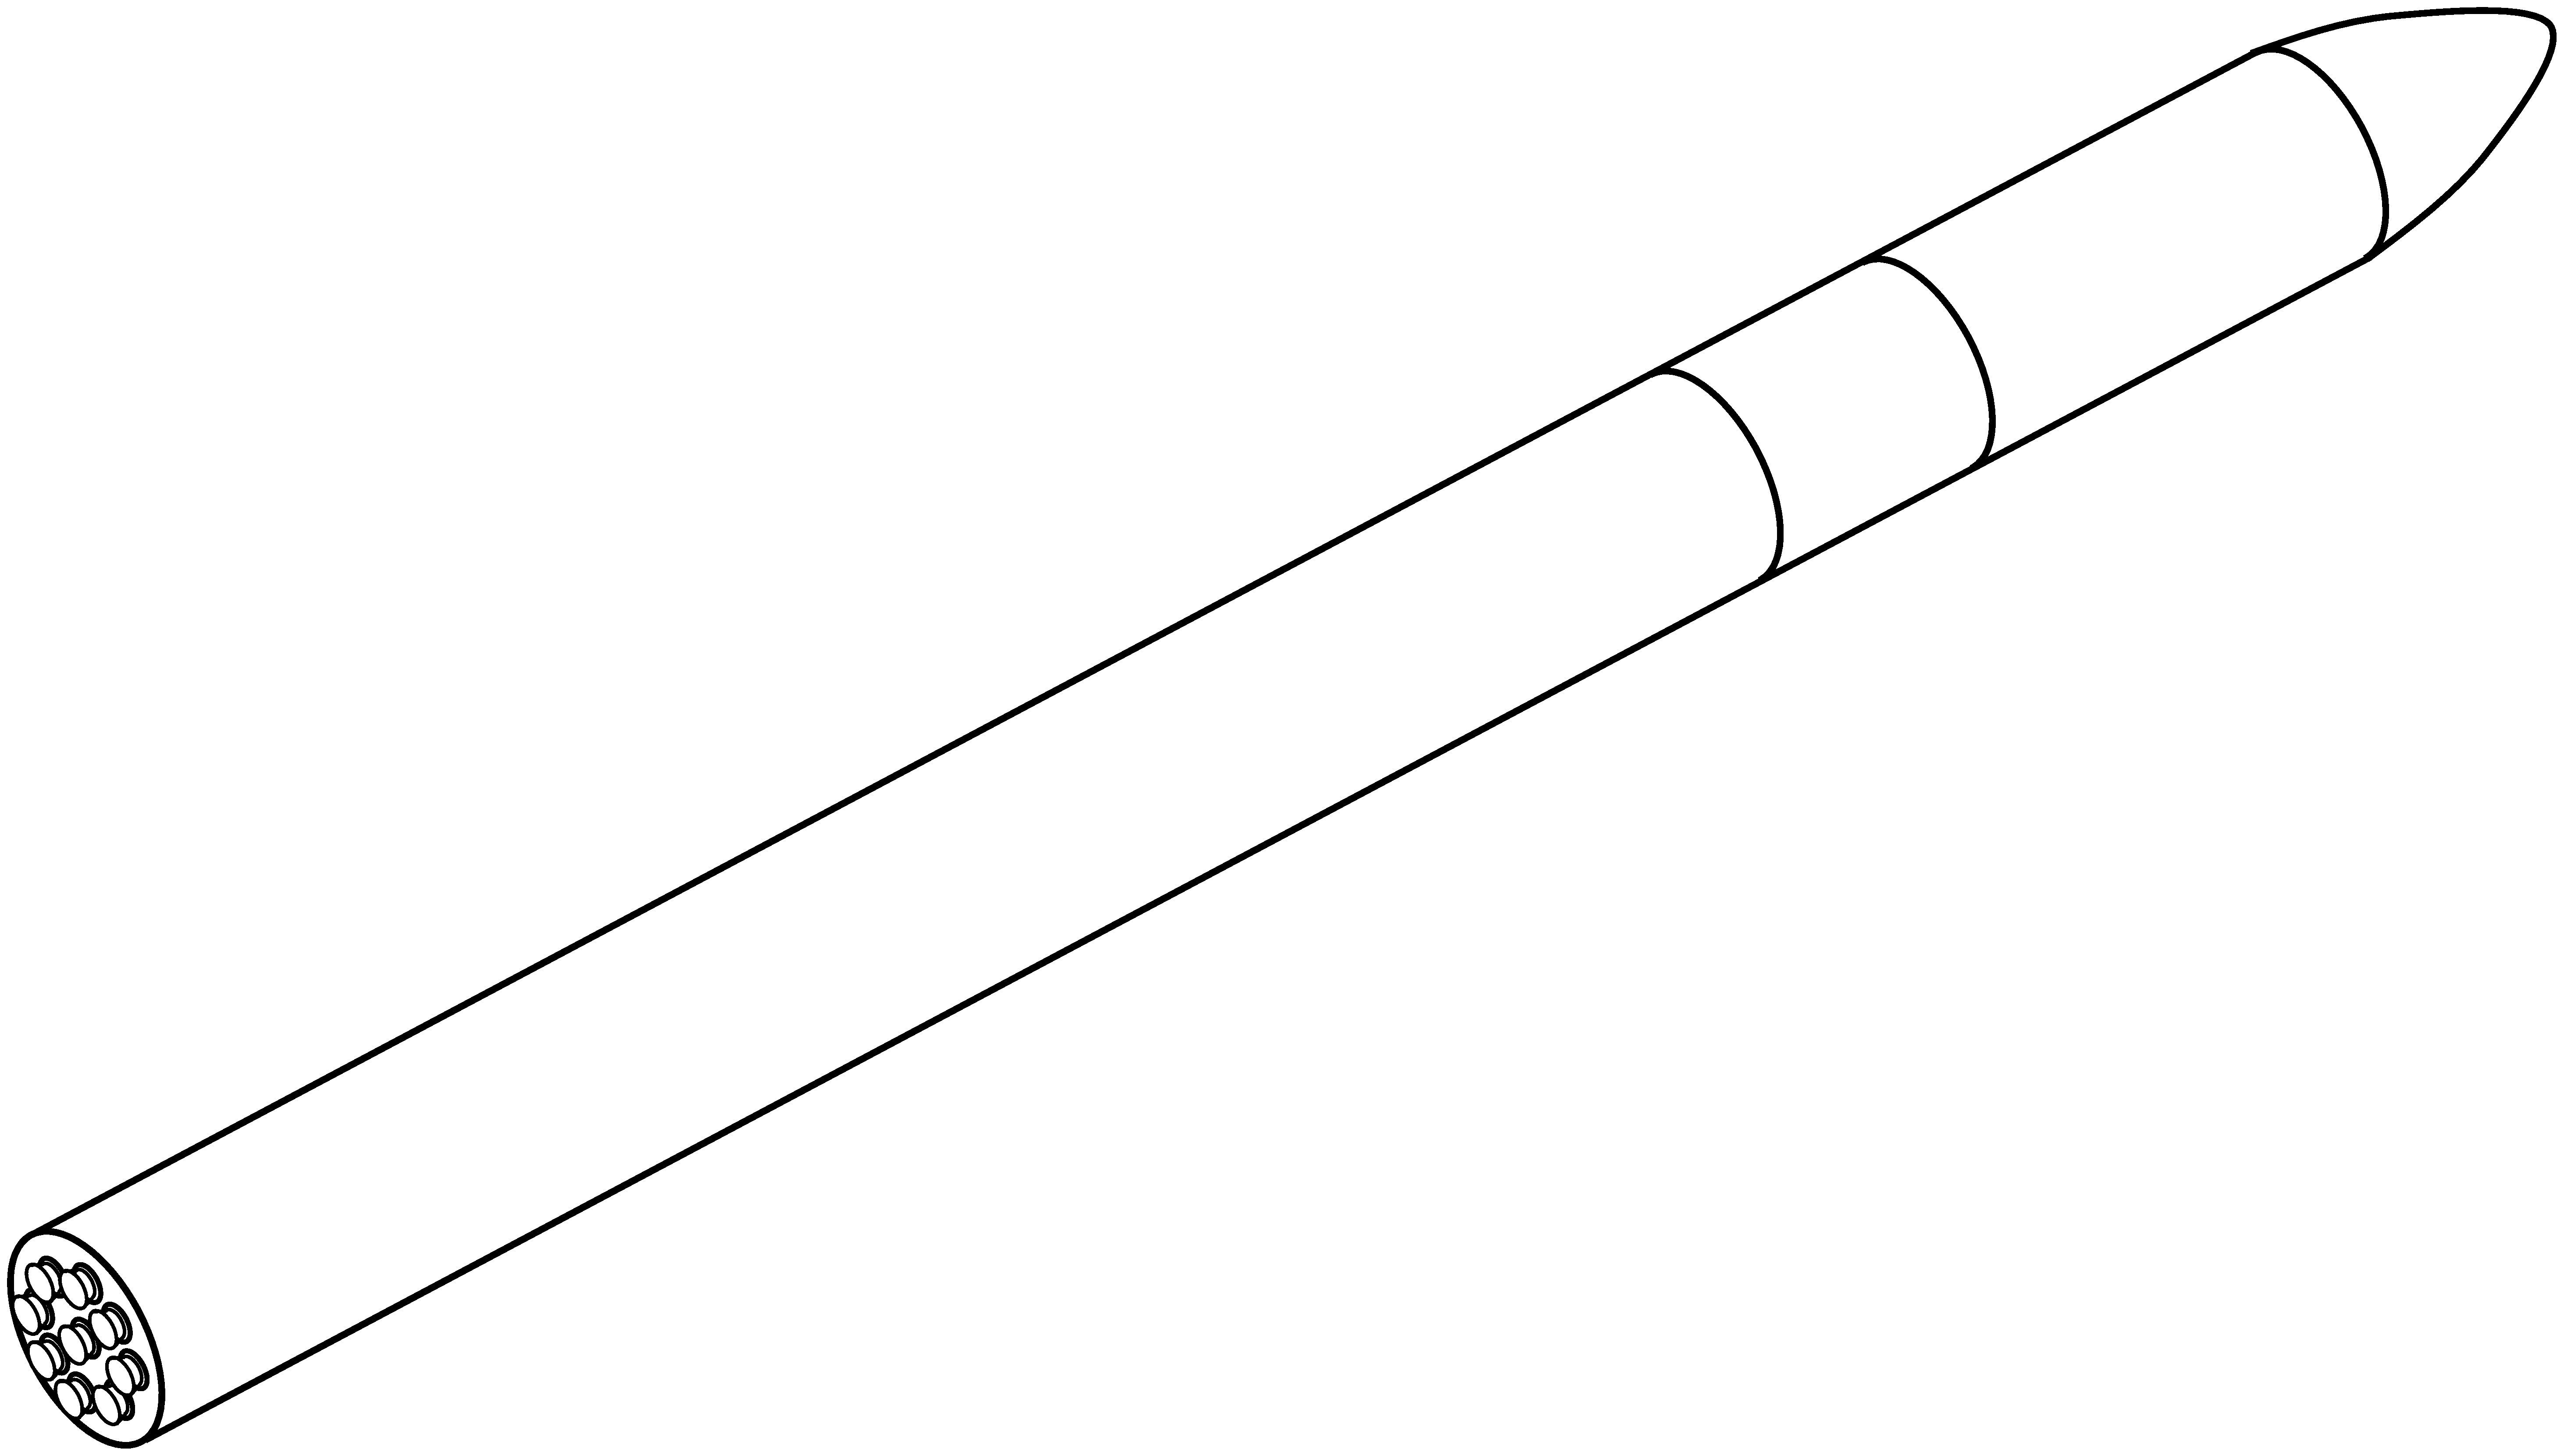
\includegraphics[width=0.6\textwidth]{../.images/rocket.eps}};
        
        % Rotation angles [deg].
        \pgfmathsetmacro{\zRot}{-30}
        \pgfmathsetmacro{\yRot}{-24.6}
        \pgfmathsetmacro{\xRot}{-25}
        
        % Scope to draw on top of rocket.
        \begin{scope}[x={(image.south east)},y={(image.north west)}]
            
            % Rotates TikZ's coordinate system to align with body frame.
            \tdplotsetrotatedcoords{\zRot}{\yRot}{\xRot}
            
            % Origin.
            \pgfmathsetmacro{\Ox}{7.5}
            \pgfmathsetmacro{\Oy}{-0.41}
            \pgfmathsetmacro{\Oz}{0}

            % Axes length.
            \pgfmathsetmacro{\axlen}{3}
            
            % Body axes.
            \draw[tdplot_rotated_coords,color_theme,line width=0.5mm](\Ox,\Oy,\Oz)--(\Ox+\axlen,\Oy,\Oz)node[pos=1.08]{$x_{b}$};
            \draw[tdplot_rotated_coords,color_theme,line width=0.5mm](\Ox,\Oy,\Oz)--(\Ox,\Oy+\axlen,\Oz)node[pos=1.1]{$y_{b}$};
            \draw[tdplot_rotated_coords,color_theme,line width=0.5mm](\Ox,\Oy,\Oz)--(\Ox,\Oy,\Oz-\axlen)node[pos=1.08]{$z_{b}$};

            % Center of mass.
            \node[draw=none,shape=circle,fill,inner sep=1.75pt,color_theme,tdplot_rotated_coords](d1)at(\Ox,\Oy,\Oz){};
            \node[xshift=-9,yshift=-5,color_theme,tdplot_rotated_coords]at(\Ox,\Oy,\Oz){$\mathrm{cm}$};

        \end{scope}

    \end{tikzpicture}

\end{document}